\documentclass[border=12pt,12pt]{standalone}
\usepackage[T1]{fontenc}
\usepackage{lmodern}
\usepackage{xcolor}
\usepackage{tikz}
\usetikzlibrary{shapes.geometric,shapes.multipart,arrows.meta,positioning,fit,calc}
\setlength{\textwidth}{16cm}
\setlength{\linewidth}{16cm}
\tikzset{
  umlclass/.style={rectangle split, rectangle split parts=3, draw, fill=white,
    font=\scriptsize, text width=5.2cm, align=left, inner sep=3pt},
  usecase/.style={ellipse, draw, fill=white, font=\footnotesize, minimum width=3.4cm,
    minimum height=0.8cm, align=center},
  act/.style={rectangle, rounded corners=6pt, draw, fill=white, font=\footnotesize,
    minimum width=4.2cm, minimum height=0.7cm, align=center},
  dec/.style={diamond, draw, fill=white, aspect=2.2, font=\scriptsize, inner sep=1pt, align=center},
  flow/.style={-{Stealth[length=2.2mm]}, thick},
  assoc/.style={-, thick},
  compo/.style={{Diamond[fill=black,length=3mm,width=2mm]}-, thick},
  aggr/.style={{Diamond[open,length=3mm,width=2mm]}-, thick},
  depend/.style={-{Stealth[length=2mm]}, dashed, thick},
  msg/.style={-{Stealth[length=2mm]}, thick},
  ret/.style={-{Stealth[length=2mm]}, dashed},
}
\newcommand{\actor}[2]{% #1 node name, #2 label
  \begin{scope}[shift={(#1)}]
    \draw[thick] (0,0.55) circle (0.18);
    \draw[thick] (0,0.37) -- (0,-0.1);
    \draw[thick] (-0.3,0.2) -- (0.3,0.2);
    \draw[thick] (0,-0.1) -- (-0.22,-0.5);
    \draw[thick] (0,-0.1) -- (0.22,-0.5);
    \node[font=\footnotesize, below] at (0,-0.5) {#2};
  \end{scope}}


\begin{document}
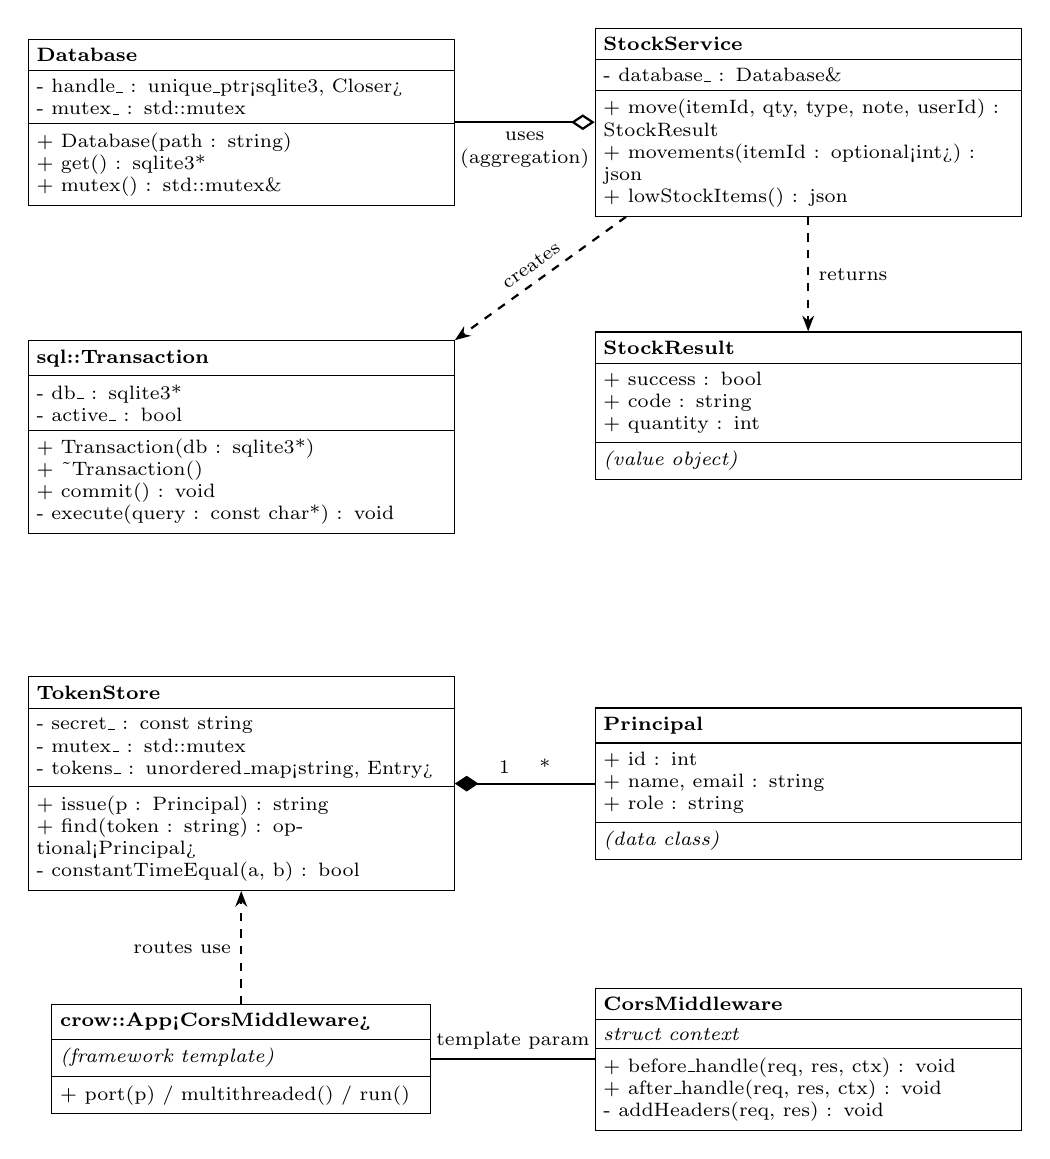
\begin{tikzpicture}[node distance=1.0cm and 0.8cm]
  \node[umlclass] (db) at (0,0) {
    \textbf{\centering Database}
    \nodepart{second}
    - handle\_ : unique\_ptr<sqlite3, Closer>\\
    - mutex\_ : std::mutex
    \nodepart{third}
    + Database(path : string)\\
    + get() : sqlite3*\\
    + mutex() : std::mutex\&};
  \node[umlclass] (ss) at (7.2,0) {
    \textbf{StockService}
    \nodepart{second}
    - database\_ : Database\&
    \nodepart{third}
    + move(itemId, qty, type, note, userId) : StockResult\\
    + movements(itemId : optional<int>) : json\\
    + lowStockItems() : json};
  \node[umlclass] (tx) at (0,-4.0) {
    \textbf{sql::Transaction}
    \nodepart{second}
    - db\_ : sqlite3*\\
    - active\_ : bool
    \nodepart{third}
    + Transaction(db : sqlite3*)\\
    + \textasciitilde Transaction()\\
    + commit() : void\\
    - execute(query : const char*) : void};
  \node[umlclass] (sr) at (7.2,-3.6) {
    \textbf{StockResult}
    \nodepart{second}
    + success : bool\\
    + code : string\\
    + quantity : int
    \nodepart{third}
    \textit{(value object)}};
  \node[umlclass] (ts) at (0,-8.4) {
    \textbf{TokenStore}
    \nodepart{second}
    - secret\_ : const string\\
    - mutex\_ : std::mutex\\
    - tokens\_ : unordered\_map<string, Entry>
    \nodepart{third}
    + issue(p : Principal) : string\\
    + find(token : string) : optional<Principal>\\
    - constantTimeEqual(a, b) : bool};
  \node[umlclass] (pr) at (7.2,-8.4) {
    \textbf{Principal}
    \nodepart{second}
    + id : int\\
    + name, email : string\\
    + role : string
    \nodepart{third}
    \textit{(data class)}};
  \node[umlclass] (cm) at (7.2,-11.9) {
    \textbf{CorsMiddleware}
    \nodepart{second}
    \textit{struct context}
    \nodepart{third}
    + before\_handle(req, res, ctx) : void\\
    + after\_handle(req, res, ctx) : void\\
    - addHeaders(req, res) : void};
  \node[umlclass, text width=4.6cm] (app) at (0,-11.9) {
    \textbf{crow::App<CorsMiddleware>}
    \nodepart{second}
    \textit{(framework template)}
    \nodepart{third}
    + port(p) / multithreaded() / run()};

  \draw[aggr] (ss.west) -- node[below, font=\scriptsize, align=center]{uses\\(aggregation)} (db.east);
  \draw[depend] (ss.south) -- node[right, font=\scriptsize]{returns} (sr.north);
  \draw[depend] ($(ss.south west)+(0.4,0)$) -- node[above, sloped, font=\scriptsize]{creates} (tx.north east);
  \draw[compo] (ts.east) -- node[above, font=\scriptsize]{1 \quad *} (pr.west);
  \draw[assoc] (app.east) -- node[above, font=\scriptsize]{template param} (cm.west);
  \draw[depend] (app.north) -- node[left, font=\scriptsize]{routes use} (ts.south);
\end{tikzpicture}
\end{document}
